% !TEX encoding = UTF-8 Unicode
%!TEX root = ../Main/thesis.tex
% !TEX spellcheck = en-US
%%=========================================
\documentclass[../Main/thesis.tex]{subfiles}
\begin{document}
\chapter[Hilbert Huang transform for high frequency pulse detection]{Hilbert Huang transform for high frequency pulse detection}
\label{sec:hht}

Most signal analysis methods such as Fourier transform, impose a-priory basis functions on the signal to be analyzed. In the case of Fourier analysis, the basis functions are trigonometric extensions. Although this implies a rigorous mathematical treatment, the resulting signal decomposition is limited by the mathematical assumptions (\cite{huang98}, \cite{huang08}). Two such assumptions are linearity and stationarity. As most phenomena in nature are non linear and non stationary, this mathematical approach, although rigorous, lacks an important property: Adaptivity (\cite{huang98}, \cite{huang08}). The latter refers to capturing the intrinsic properties of a signal, without imposing a-priory basis functions, (\cite{huang98}, \cite{huang08}). 
\justify 
The Hilbert Huang transform (HHT) was precisely developed to deal with non linear and non stationary processes, in an adaptive fashion (\cite{huang98}). It combines Hilbert spectral analysis with the so call empirical mode decomposition (EMD), to adaptively decompose a signal into its fundamental components called intrinsic mode functions (IMF), (\cite{huang98}).
The richness of the HHT spans from the analysis of differential equations, to the study of geophysical phenomena, as well as bearings faults detection (\cite{huang08},\cite{li2009}, \cite{yan2006} ,\cite{soualhi2015}, \cite{sallo2019}), and by no mean limited to them.
\justify
 The HHT has been successful applied to the analysis of solutions of nonlinear differential equations, such as the Duffing and the Lorentz equations. The intrinsic frequency, the forcing function and the low intensity subharmonics of the numerical solutions for the nonlinear Duffing equation has been extracted through the EMD process, (\cite{huang98}).
 \justify
  The decomposition of the solutions of Lorentz equation, revealed \say{transient components with different frequencies and damping characteristics}, which agreed with previous studies, (\cite{huang98}). The HHT application to seismic waves propagation, made it possible to identified high and low frequency seismic waves (\cite{vasudevan2000}). In particular, its decomposition of the seismic waves induced by the 1999 Taiwan earthquake, revealed that \say{the Fourier transform underestimated low frequency energy} (\cite{huang2001}). 
\justify
The Hilbert Huang transform emerged as a general signal decomposition tool, and in theory can be applied to any signals.
This chapter presents a new method for bearing fault detection. The method couples the HHT with a robust seasonal trend decomposition method called STL, to detect bearing faults. STL stands for seasonal trend decomposition based on LOESS. In short, the STL decomposes a target signal into a trend and an oscillatory component also called  seasonality. The trend is a monotone curve, while the seasonality is periodic.
The bulk of this new method, consists of extracting the seasonality, from the Hilbert Huang transform of a bearing vibration signal. The idea is that the seasonality component which is a pulse like signal, contains all the diagnostic information in terms of bearings failure frequencies.
\justify
After giving an esquisse of the new method, the remaining of this chapter is organized in the following manner:
 Section \ref{sec:emd} presents the empirical mode decomposition (EMD), which is the back bone of the Hilbert Huang transform for decomposing a signal adaptively.
 Section \ref{sec:pulse}, through a concrete case study, shows that the HHT, coupled with the STL, are able to recover the high frequency pulse like signals, emitted by bearing defects. The section starts by recalling the characteristics of two bearing faults: The outer race defect and the inner race defect. Furthermore, the experiments that generated the data for this case study are described. Afterwards, the seasonal trend decomposition based on LOESS (STL) is presented, followed by a description of the proposed method for bearing fault detection. Finally, the results of the application to the case study are presented. In closing, section \ref{sec:limitation} presents a summary and discussion of the proposed new method.
\justify
\section{Hilbert Transform}
\label{sec:ht}

The Hilbert transform is an import tool in mathematics, and in signal processing in particular. Among others, its makes possible the representation of a real valued signal as an analytic signal (a complex signal), which is its extension to the upper half complex plane. By doing so, the concept of instantaneous amplitude and instantaneous frequency can be introduced, which is important in amplitude and frequency modulation problems [picinbono1989], such as transmission of radio communication signals, analysis of vibration signals under varying load, etc. Here amplitude and frequency modulation refers to the time dependency of the amplitude and the frequency. In the formulation of Fourier analysis, the frequency and amplitude of a signal are constant. However, in many  practical problems, amplitude and frequency modulation are imposed.
\justify
 Before moving to the mathematical formulation of the Hilbert transform, let define an analytical signal.
 Formally, an analytical signal is a complex signal whose imaginary part is the Hilbert transform of its real part. A real valued signal $x(t)$ , can be extended to a well defined complex signal $s(t)$, 
 \begin{equation}\label{eq:ana}
 	s(t) = x(t) + i H\{ x(t)\}
 \end{equation}
where $H\{ x(t)\}$ is the Hilbert transform of $x(t)$. The signal $s(t)$ is well defined in the sense that its existence and uniqueness are guaranteed. If (\ref{eq:ana}) holds, then $s(t)$ is said to be an analytical signal. Furthermore, if $s(t)$ is a mono-component signal, its amplitude $a(t)$ and frequency $\omega(t)$ as a function of the time variable $t$ are given by

%As any new methods, the Hilbert Huang transform strives in improving upon previous signal processing paradigms. It rests on adaptivity, non linearity, non stationarity and physical meaningful time-frequency-energy paradigm. The latter is akin to the fundamental concept of uniqueness in the study of the solution of differential equations. 
%In Fourier analysis, a time dependent signal $S(t)$, can be expressed as the following complex expansion
%\begin{equation} \label{eq:fourier}
%S(t) = \sum_{j=1}^{\infty}a_{j}\exp(i\omega_{j}t),
%\end{equation}
%where $a_{j}, \omega_{j}$ are constant amplitudes and frequencies respectively, and $i = \sqrt{-1}$. The Hilbert Huang transform generalizes the Fourier expansion (\ref{eq:fourier}) with time dependent amplitude $a(t)$ and frequency $\omega(t)$ as 
%\begin{equation} \label{eq:hht}
%S(t) = \sum_{j=1}^{n}a_{j}(t)\exp\left(i\int \omega_{j}(t)\mathrm{dt}\right).
%\end{equation}
%Equation (\ref{eq:hht}) expresses non stationarity as opposed to equation (\ref{eq:fourier}), by providing amplitude and frequency modulation. Here amplitude and frequency modulation refer to the time dependency of the amplitude $a(t)$ and the frequency $\omega(t)$. The former and the latter can be derive through the Hilbert transform. let $H(t)$ be the Hilbert transform of the signal $S(t)$ and given by
%\begin{equation}\label{eq:hilbert}
%H(t) = \frac{P}{\pi}\int_{-\infty}^{\infty}\frac{S(\tau)}{t-\tau}\mathrm{d\tau},
%\end{equation}
%where $P$ is the Cauchy principal value of the singular integral (\cite{huang08}). The amplitude $a(t)$ and the frequency $\omega(t)$

\begin{equation}\label{eq:amplitude}
a(t) = \sqrt{x(t)^{2} + H\{x(t) \}^{2} }
\end{equation}
\begin{equation}\label{eq:frequency}
\omega(t) = \frac{d \Psi(t)}{dt} 
\end{equation}
where 
\begin{equation}\label{eq:frequency}
\Psi(t) = \tan^{-1}\left(\frac{H\{x(t) \}}{x(t)} \right),
\end{equation}
is the instantaneous phase. With these formulations, $s(t)$ can be expressed simultaneously in the time and frequency domain (a mixed representation) as 
\begin{equation}\label{eq:modulation}
	s(t) = a(t)\cos\left( \Psi(t)\right) 
\end{equation}
Recall that a mono-component signal is a signal with no other frequency component then its own.
In contrast to (\ref{eq:modulation}), the Fourier analysis represents a signal either in time or in frequency domain, where the concept of instantaneous frequency and amplitude can not be defined. The amplitude and frequency modulation expressed in (\ref{eq:modulation}) gives a correct representation of signals which are non periodic, where obviously the frequency and the amplitude varies continuously with time.
\justify
The Hilbert transform $H\{ x(t) \}$ of a signal $x(t)$, is define as its convolution with the function $\frac{1}{\pi t}$ expressed as
\begin{equation}\label{eq:conv}
H\{ x(t) \} = \frac{1}{\pi t}* x(t) = 	\frac{1}{\pi}P \int_{-\infty}^{\infty}\frac{x(\eta)}{t-\eta}\mathrm{d\eta}.
\end{equation}
Because of the pole at $t=\eta$ in (\ref{eq:conv}), the indefinite integral might not converge. To circumvent this issue, the indefinite integral is evaluated by applying the Cauchy principal value method, as indicated by the letter $P$ in front the integral. Furthermore (\ref{eq:conv}), can be written as
\begin{equation}
	\begin{split}
	H\{ x(t) \} &=  \frac{1}{\pi}P \int_{-\infty}^{\infty}\frac{x(\eta)}{t-\eta}\mathrm{d\eta}\\
				&= \frac{1}{\pi}\lim_{\epsilon\rightarrow 0^{+}} \left( \int_{-\infty}^{-\epsilon} \frac{x(\eta)}{t-\eta}\mathrm{d\eta} +   \int_{\epsilon}^{\infty} \frac{x(\eta)}{t-\eta}\mathrm{d\eta}     \right)
	\end{split}
\end{equation}

\begin{figure}[H]
	\centering
	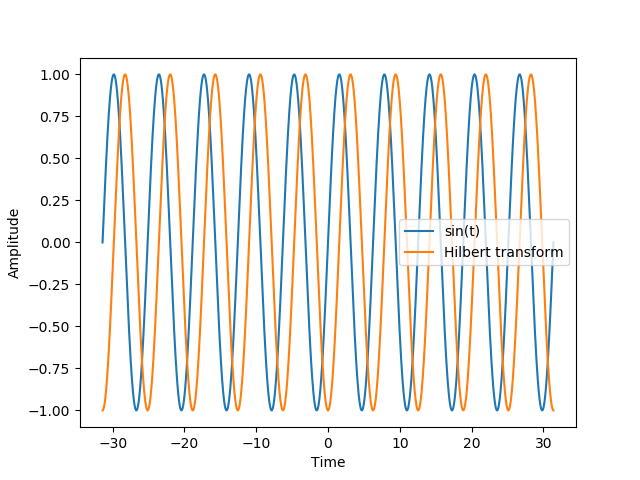
\includegraphics[width=0.8\linewidth]{../fig/h_sin}
	%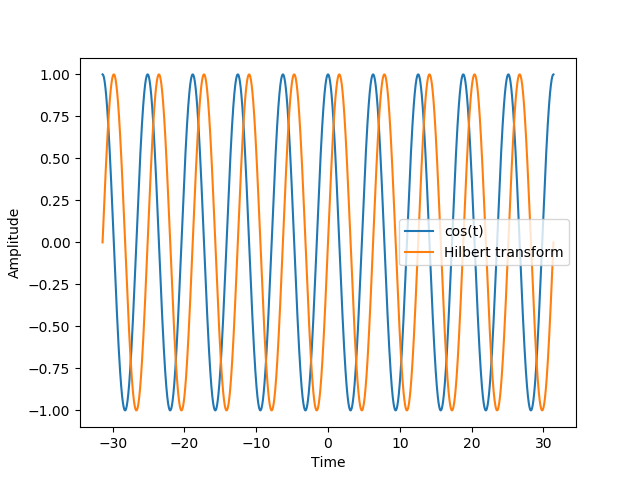
\includegraphics[width=0.8\linewidth]{../fig/h_cos}
	\caption{The Hilbert transform of $\sin(ct)$ given by $\sin(ct-\frac{\pi}{2})$. $c=1$  }
	\label{fig:hsin}
\end{figure}
\justify
Figure \ref{fig:hsin} shows the Hilbert transform of $\sin(ct)$ which is $\sin\left(ct-\frac{\pi}{2}\right)$. In the same fashion, the Hilbert transform of $\cos(ct)$ is  $\cos\left(ct-\frac{\pi}{2}\right)$, where $c = 1$. As a consequence, the Hilbert transform imposes a phase shift of $\frac{\pi}{2}$ to every Fourier component of a signal. Figure \ref{fig:cauchy_pulse} and \ref{fig:sinc_pulse} show the Cauchy pulse $\left(\frac{c}{c^{2} + t^{2}}\right)$ and the sinc pulse $\left(\frac{\sin(ct)}{ct}\right)$ with their corresponding Hilbert transform for $c = 1.5$.
\begin{figure}[H]
	\centering
	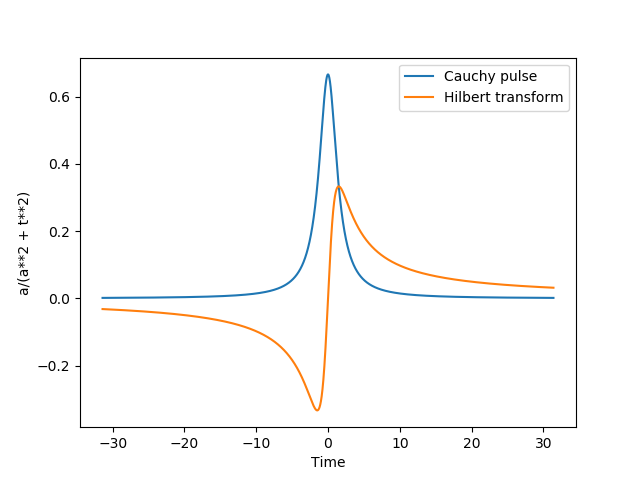
\includegraphics[width=0.8\linewidth]{../fig/cauchy_pulse}
	\caption{The Hilbert transform of Cauchy pulse }
	\label{fig:cauchy_pulse}
\end{figure}

\begin{figure}[H]
	\centering
	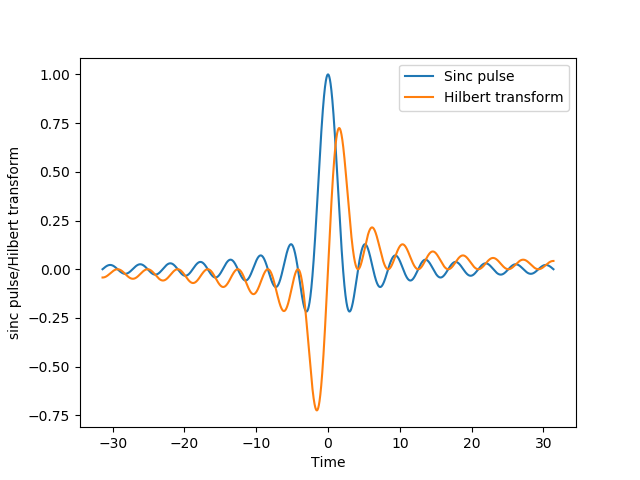
\includegraphics[width=0.8\linewidth]{../fig/sinc_pulse}
	\caption{The Hilbert transform of Cauchy pulse }
	\label{fig:sinc_pulse}
\end{figure}
\justify
The amplitude and frequency modulation obtained from Hilbert transform in equation (\ref{eq:amplitude}, \ref{eq:frequency}) does not always provide a meaningful (well defined) physical description of a signal unless the signal is mono-component (\cite{huang98}, \cite{huang08}). The Hilbert Huang transform was developed to tackle this issue. Through the so called empirical mode decomposition (EMD), which is a series of transformation, a target signal is decomposed into (nearly) mono-component signals called intrinsic mode function, for which instantaneous amplitude and frequency are well defined in a physical sense.



 
 
 \section{Hilbert Huang transform}
 \label{sec:emd}
  The empirical mode decomposition (EMD), decomposes a given signal into sub-components call intrinsic mode functions (IMFs), such that every IMF produces physically meaningful amplitude and frequency modulation, (\cite{huang98}).
 For a target signal $S(t)$, the goal is to obtained its $n$ fundamental parts (IMFs), denoted here by $s_{j}, j =1,\cdots,n$, through the empirical mode decomposition, such that
\begin{equation}\label{eq:emd-decomposition}
S(t) = \sum_{j=1}^{n}s_{j}(t) + r(t),
\end{equation}
where $r(t)$ is the residual, which is either a constant or a monotone function. The derivation of the intrinsic mode functions $s_{j}$, by means of the empirical mode decomposition, relies on the following key assumptions.
\begin{definition}\label{def:emd}
An intrinsic mode function (IMF) must satisfy the following conditions:
\begin{enumerate}
\item The number of extrema and the number of zero crossing must either equal or differ by one 
\item At any data point, the mean value of the envelope defined using the local maxima and the envelope defined by using the local minima is zero.
\end{enumerate}
\end{definition}
The empirical mode decomposition is an iterative algorithm that generates intrinsic mode functions, each satisfying definition \ref{def:emd}.
\justify
The empirical mode decomposition can be described as follow:
\begin{enumerate}
	\item Compute the upper and the lower envelope curve of the target signal $S(t)$
	\item In the first iteration $i=1$, compute the mean $m_{i}(t)$ between the upper and the lower envelope cure of $S(t)$
	\item Compute the fist pseudo IMF as 
	\begin{equation}\label{eq:proto}
		h_{i1}(t) = S(t)-m_{i}(t).
	\end{equation}
	If $h_{i1}$ satisfies definition \ref{def:emd}, then it is an IMF and it is denoted by 
	\begin{equation}\label{eq:imf}
		c_{i}(t) = h_{i1}(t).
	\end{equation}
	otherwise
	
	\item Set $h_{i1}(t)$ as the input signal and repeat step 1,2 and 3, $k$ time, until $h_{ik}(t)$ satisfies definition \ref{def:emd}.
	\item After finding the first IMF, set the first IMF as input signal and repeat step 1,2,3 and 4 to obtain the remaining IMFs. If an IMF is monotone, set it as the residual and you are done.
\end{enumerate}
Figure \ref{fig:emd3} shows the the signal  $S(t) = \sin(10 \pi t) + \sin(20 \pi t) $ (top) and its IMFs as well as the residual. In most function approximation methods, a set of basis functions $\varphi_{j}(t), j = 1,\cdots,n$ coupled with coefficients $a_{j}$, are used to decomposing a function $f(t)$ as 
\begin{equation}\label{eq:basis}
	f(t) = \sum_{j=1}^{n}a_{j}\varphi_{j}(t).
\end{equation}
However, the Hilbert Huang transform will decompose $f(t)$ as 
\begin{equation}\label{eq:hht1}
f(t) = \sum_{j=1}^{n}c_{j}(t) + r(t).
\end{equation}
In equation (\ref{eq:basis}) the basis $\varphi_{j}(t)$ are chosen before hand (a-priory), and the coefficients are computed through an integral or summation operation. A sort of \say{bias} is imposed on the the function $f(t)$. On the hand, in equation (\ref{eq:hht1}) one can clearly state that the basis function are directly computed based on the function $f(t)$. This illustrates the concept of adaptivity, central to the Hilbert Huang transform.
\begin{figure}[H] %  figure placement: here, top, bottom, or page
   \centering
   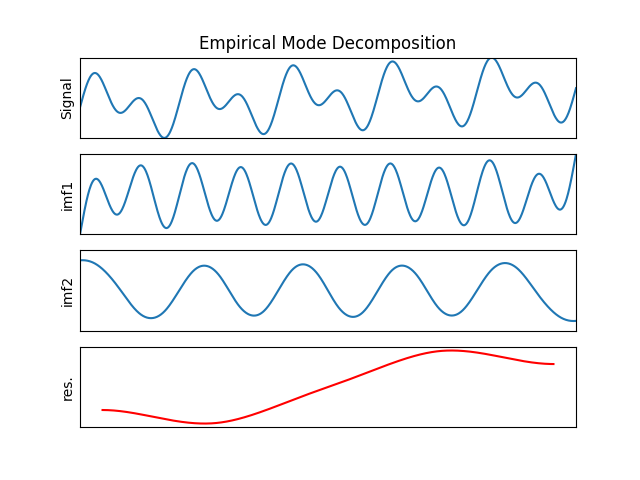
\includegraphics[width=6in]{../fig/imfEMD.png} 
   \caption{The intrinsic mode functions (IMF ) and the residual (in red) generated from the input signal $S(t) = \sin(10 \pi t) + \sin(20 \pi t) $}
   \label{fig:emd3}
\end{figure}
\justify
The intrinsic mode functions obtained through the EMD process constitute an adaptive basis that satisfies the mathematical properties of convergence, completeness, orthogonality and uniqueness, (\cite{huang98}). Furthermore, if $a_{j}(t)$ and $\omega_{j}(t)$ are amplitude and frequency modulation corresponding to IMF $j$, then the original signal $S(t)$ can also be recover as 
\begin{equation}\label{eq:recover2}
S(t) = \Re{\left( \sum_{j=1}^{n}a_{j}(t)\exp\left(i\int\omega_{j}(t)\mathrm{dt}\right)  \right)},
\end{equation} 
where the symbol $\Re(\cdot)$ represents the real part of the expression its encompasses, $i=\sqrt{-1}$, and $n$ is the total number of IMFs obtained from decomposing a signal $S(t)$. Recall that the amplitudes $a_{j}(t)$ and the frequencies $\omega_{j}(t)$ can be computed through the Hilbert transform from equations (\ref{eq:hilbert}, \ref{eq:amplitude}, and \ref{eq:frequency}). An analog representation of equation (\ref{eq:recover2}) in terms of Fourier expansion would be 
\begin{equation}\label{eq:recoverFourier}
S(t) = \Re{\left( \sum_{j=1}^{n}a_{j}\exp\left(i\omega_{j}\right)  \right)},
\end{equation} 
where this time, the amplitude $a_{j}$ and the frequency $\omega_{j}$ are constant. The Hilbert Huang transform (HHT) offers two different approaches to recover a decomposed signal. The first one is described by equation (\ref{eq:hht1}) and include the IMFs, while the second approach is given by equation (\ref{eq:recover2}) and includes the instantaneous amplitude and the instantaneous frequency. This gives the HHT a leverage over Fourier transform in nonlinear an non stationary data analysis.
%%%%%%%%%%%%%%%%%%%%%%%%%%%%%%%%%%%%%%%%%%%%%%%%%%%%%%%%%%%%%%%%%%%%%%%%%%%%%%%%%%%%%
%%%%%%%%%%%%%%%%%%%%%%%%%%%%%%%%%%%%%%%%%%%%%%%%%%%%%%%%%%%%%%%%%%%%%%%%%%%%%%%%%%%%%
%%%%%%%%%%%%%%%%%%%%%%%%%%%%%%%%%%%%%%%%%%%%%%%%%%%%%%%%%%%%%%%%%%%%%%%%%%%%%%%%%%%%%

\section{Application of the Empirical mode decomposition to pulse detection}
\label{sec:pulse}
After introducing the Hilbert Huang transform in the previous section, we are now ready to apply the empirical mode decomposition to a case study: Detecting pulses emitted by a bearing with crack in the outer and inner ring. First of all, a few recalls: Figure \ref{fig:bearing-architecture} shows a geometry of a bearing, with different parts.
\begin{figure}[H] %  figure placement: here, top, bottom, or page
   \centering
   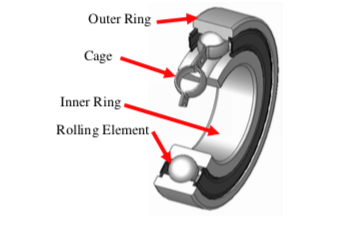
\includegraphics[width=4in]{../fig/bearing.png} 
   \caption{Geometrical representation of a bearing}
   \label{fig:bearing-architecture}
\end{figure}
\justify
A fault occurring at the outer ring is called a ball pass frequency outer ring (BPFO) defect. While a fault in the inner ring occurs at a frequency called ball pass inner race frequency (BPFI). They are given in Hz in terms of the bearing geometrical characteristics an the rotating speed of the shaft as
\begin{equation}\label{eq:bpfo2}
BPFO = \frac{nb}{2}R\left(1-\frac{BD}{PD}\cos\left(\beta\right)  \right) \nonumber,
\end{equation}
\begin{equation}\label{eq:bpfi2}
BPFI = \frac{nb}{2}R\left( 1 +  \frac{BD}{PD}\cos\left(\beta\right)   \right)
\end{equation}
where R is the rotating speed of the motor on which the bearing is attached. nb is the number of rolling elements (balls), BD is a rolling element diameter. The pitch diameter PD is half the hight of the inner ring, and the contact angle $\beta$ is the angle formed when a rolling element touches the cage. 
\justify
The data and the experimental setup used for this case study were described in chapter 2. In this setup, four bearings are mounted on a motor rotating at 2000 rotations per minutes (33.3 Hz). In the first experiment the motor runs until bearing
bearing number 3 is severely damaged with inner race defect, while in the second experiment outer race defect occurs in bearing number 1. For each experiment, successive vibration signals where obtained, with a sample rate of 20 $KHz$ and corresponding Nyquist frequency of 10 $KHz$ (half the sampling rate). The Nyquist frequency define a lower bound limit in order to avoid aliasing, which is a loss of information due to under sampling. That is, if the sample contain frequency components that are higher then the Nyquist frequency, those frequency component wont be able to be seen.

\justify
\subsection{Seasonal Trend decomposition based on Loess (STL)}
The STL sequentially applies the locally estimated scatter plot smoother (LOESS) in order to obtain cyclical and trend components of a signal (\cite{Cleveland-1979}, \cite{Cleveland-et-al-1988}). Here a cyclical component is a periodically occurring pattern in a signal. The  locally estimated scatter is a non parametric curve fitting procedure.  It can be used for \say{Data exploration, diagnostic checking of parametric models and provides a non parametric regression surface}.
If $S(t)$ is a signal, the goal is to obtained the decomposition 
\begin{equation}
S(t) = T_{r}(t) + C_{y}(t) + R_{res}(t),
\end{equation} 
where $T_{r}(t)$ an $C_{y}(t)$ are the trend and cyclical components, and $R_{res}(t)$ is the residual obtained from subtracting  the trend and the cyclical component from the signal. The key ingredient in the STL, is the locally estimated scatterplot smoother procedure. The latter being a non parametric regression method, does not rely on any a-priory assumption on the shape of the curve that needs to be fitted. Its therefore provides a flexible approach to curve fitting, by capturing local, as well as global characteristics of a signal. Since pulses emitted by a bearing roller elements passing a crack, are local periodic events on a global scale, the STL provides the necessary mathematical apparatus to capture them. A detailed account of the STL can be found in  (\cite{Cleveland-et-al-1990}).

\justify
%By design, the STL is computational efficient, robust in the sense that it uses a robust statistical estimator, and deals very well with missing and distorted data points (\cite{Cleveland-et-al-1990}). In the subsequent paragraphs, an account of the LOESS procedure is presented.
%\justify
%Given a signal represented by a set of $n$ points, conveniently expressed by their coordinates
%\begin{equation}
%\{ (t_{j}, y_{j}), \quad j = 1, \cdots, n\},
%\end{equation}
%where $t_{j}$ is the independent variable on the time scale, and $y_{j}$ is the dependent variable. The LOESS procedure finds a smooth function $\hat{g}(t)$, defined everywhere on the scale of the independent variable, such that the estimate of $y_{j}$ denoted by $\hat{y}_{j}$ at $t_{j}$ is computed as 
%\begin{equation}
%\begin{split}
%\hat{y}_{j} &= \hat{g}(t_{j}) \\
%                &=\sum_{k=0}^{d}\hat{\alpha}_{k}(t_{j})t_{j}^{k}
%\end{split}
%\end{equation}
%where the $\hat{\alpha}_{k}(t_{j})$ are the values $\alpha_{k}$ that minimize 
%\begin{equation}
%\sum_{k=1}^{n}w_{k}(t_{j})\left(y_{k}-\alpha_{0}-\alpha_{1}t_{k}-\cdots -\alpha_{d}t_{k}^{d}\right)^{2}
%\end{equation}
%with 
%\begin{equation}
%w_{k}(t_{j}) = W\left( \frac{t_{k}-t_{j}}{h_{j}} \right)
%\end{equation}
%
%\begin{equation}
%W(t) = 
%  \begin{cases}
%  \left(1-t^{3}\right)^{3} &\quad\text{for } 0\leq t \le 1\\
%   0 &\quad\text{for} t\geq 1
% \end{cases}
%\end{equation}
%and $h_{j}$ is the distance from $t_{j}$ to the nearest neighbor of $t_{j}$. 



%%%%%%%%%%%%%%%%%%%%%%%%%%%%%%%%%%%%%%%%%%%%%%%%%%%%%%%%%%%%%%%%%%%%%%%%%%%%%%%%%%%%%%%%%%%%%%
%%%%%%%%%%%%%%%%%%%%%%%%%%%%%%%%%%%%%%%%%%%%%%%%%%%%%%%%%%%%%%%%%%%%%%%%%%%%%%%%%%%%%%%%%%%%%%

\subsection{Results from applying empirical mode decomposition and seasonal trend decomposition base on Loess}
In this section we apply the empirical mode decomposition followed by the seasonal trend decomposition based on LOESS to extract pulses emitted by a failed bearing.
Figure \ref{fig:pulse} shows a flow diagram, describing the methodology to obtaining pulse signals emitted from a bearing with ball pass frequency outer race defect. An input signal goes through the empirical mode decomposition to generate intrinsic mode functions. Furthermore, the STL is applied on the intrinsic mode functions to generate a periodic signal which looks like a pulse.

\begin{figure}[H]
\begin{tikzpicture}
  [node distance=.8cm,
  start chain=going below,]
     \node[punktchain, join] (intro) {\textcolor{blue}{Input signal}};
     \node[punktchain, join] (probf)      {\textcolor{violet}{EMD}};
     \node[punktchain, join] (investeringer)      {\textcolor{blue}{IMFs}};
     \node[punktchain, join] (perfekt) {\textcolor{violet}{STL}};
     \node[punktchain, join] (perfekt) {\textcolor{blue}{Pulse signal}};
     %\node[punktchain, join, ] (emperi) {Fast Fourier transform};
     % \node (asym) [punktchain ]  {Asymmetrisk information};
      \begin{scope}[start branch=venstre,
        %We need to redefine the join-style to have the -> turn out right
        every join/.style={->, thick, shorten <=1pt}, ]
        \node[punktchain, on chain=going left, join=by {->}] (risiko) {\textcolor{blue}{Power spactrum density}};
      \end{scope}
      \begin{scope}[start branch=hoejre,]
      %\node (finans) [punktchain, on chain=going right] {Det finansielle system};
    \end{scope}
    \end{tikzpicture}
  \caption{Schematic description of the methodology to obtaining a pulse like signal containing all diagnostic information for bearing fault detection}
   \label{fig:pulse}
\end{figure}
\justify
The power spectral density of the resulting signal is approximated by a periodogram, which is the representation of the energy distribution of the most compelling frequency components in the signal. Recall that the power spectral density is the energy distribution of frequencies of a signal. The periodogram shows peaks that correspond to strong sinusoidal components. Some of the strong sinusoidal components that we expect to see are the bearing defect frequencies and the rotation frequency of the machine shaft.

\begin{figure}[H] %  figure placement: here, top, bottom, or page
	\centering
	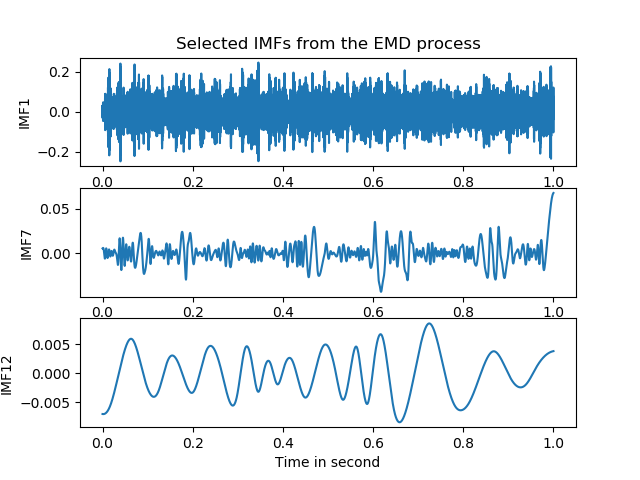
\includegraphics[width=6in]{../fig/selected_imf.png} 
	\caption{Intrinsic mode function number 1, 7 and 12, generated by the empirical mode decomposition}
	\label{fig:imf}
\end{figure}
\justify
Figure \ref{fig:imf} shows three selected intrinsic mode functions (IMFs) generated by the empirical mode decomposition. The first IMF is a high frequency signal, while IMF number 7 and 12 are relatively low frequencies signals.
\begin{figure}[H] %  figure placement: here, top, bottom, or page
   \centering
   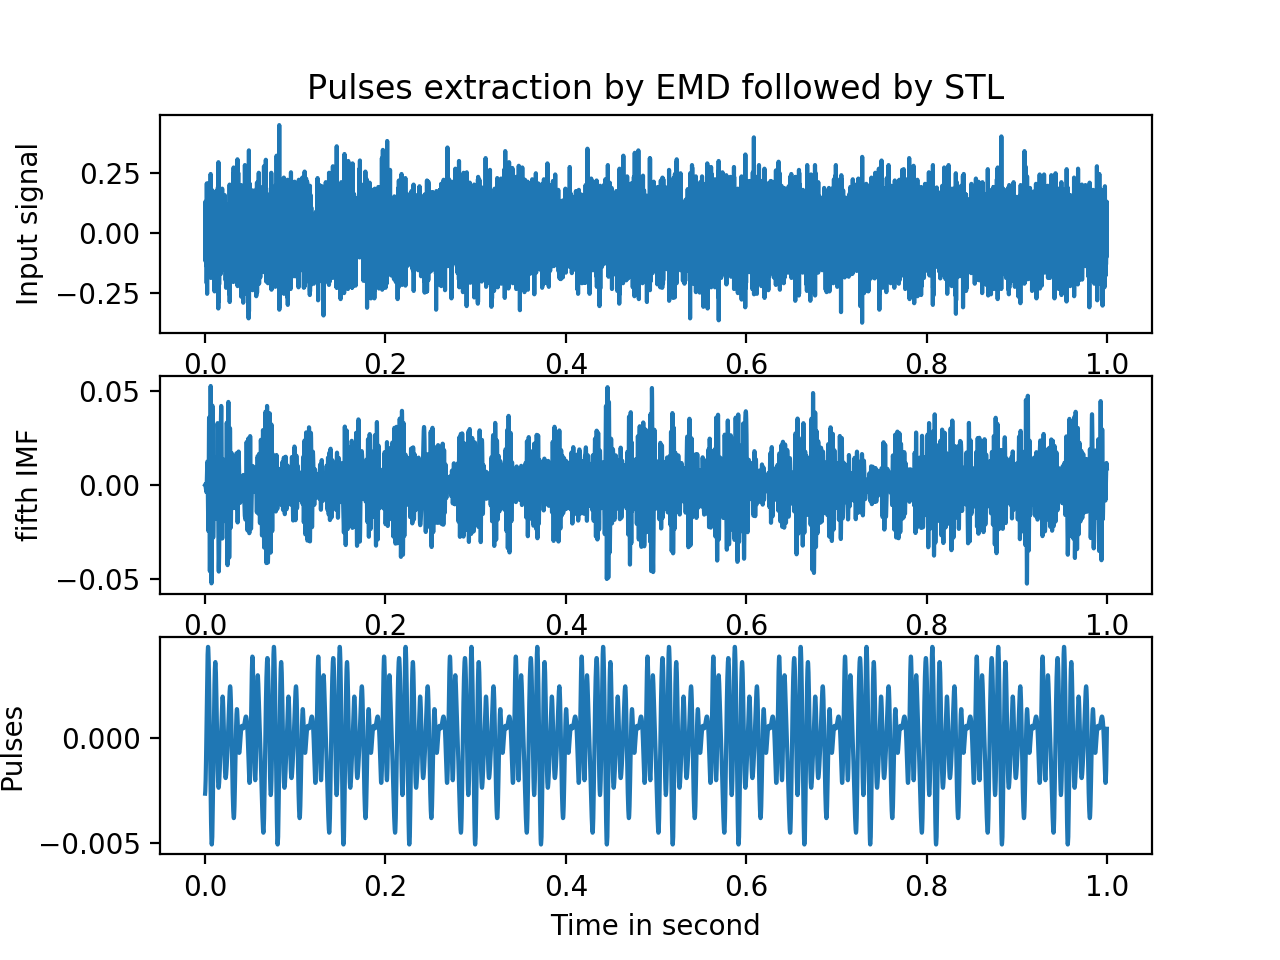
\includegraphics[width=6in]{../fig/emd-stl.png} 
   \caption{ A pulse signal extracted by applying EMD followed by STL. The top graph represents the vibration time signal. The middle graph is the fifth intrinsic mode function. The bottom graph is the signal resulting from applying the STL on the IMF. The pulses represents the periodic high frequency signal emitted by bearings defects.}
   \label{fig:emd-stl}
\end{figure}
\justify
Figure \ref{fig:emd-stl} shows, the result from applying the EMD and the STL to an input signal. The top graph represents the input vibration signal. The middle graph shows the fifth intrinsic mode function obtained from applying the Hilbert Huang transform. The bottom graph is a signal resulting from applying the STL on the fifth intrinsic mode function. It is a periodic pulse like signal.

\subsubsection{Ball pass frequency outer race detection} 
%The middle graph shows the fifth intrinsic mode function generated from applying the EMD on the input signal. This IMF shows patterns.
%This is precisely what is require to capture a pulse, which can be viewed as a periodic emanation of an event such as a bearing ball passing a crack.
 \begin{figure}[H]
 	\centering
 	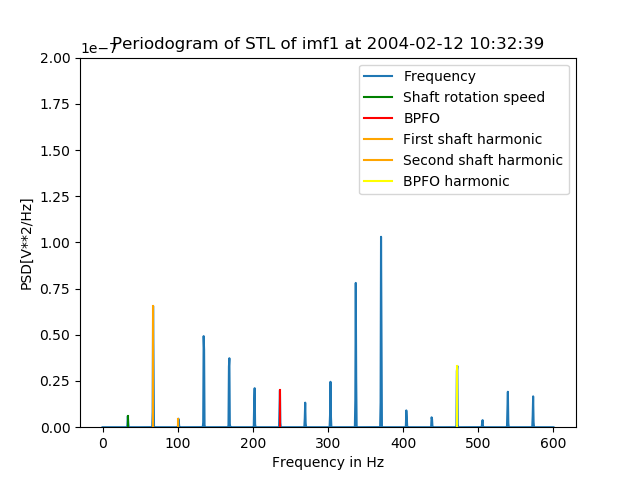
\includegraphics[width=0.8\linewidth]{../fig/periodogram_bpfo/start_imf1_bpfo}
 	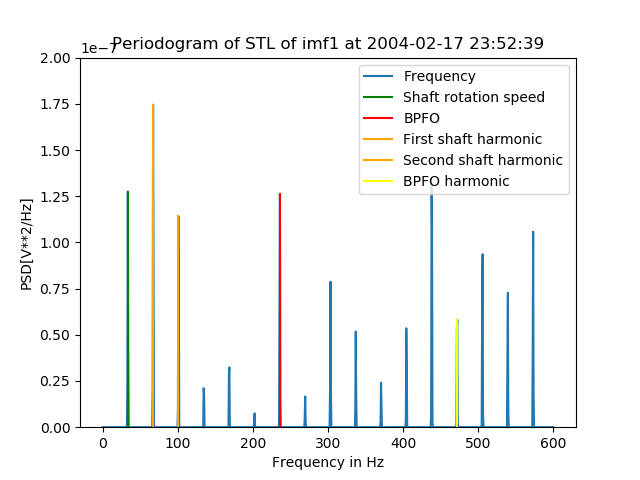
\includegraphics[width=0.8\linewidth]{../fig/periodogram_bpfo/end_imf1_bpfo}
 	\caption{Periodogram of the pulse signal obtained from the first IMF, at the beginning (top) and the end (bottom) of experiment number 2}
 	\label{fig:startimf1bpfo}
 \end{figure}
\justify
Figure \ref{fig:startimf1bpfo} shows the periodogram of the pulse signal of the first IMF obtained at the beginning (top) and at the end of experiment number 2. The shaft frequency (33 Hz) and its first and second harmonics are clearly visible.
The ball pass outer race frequency defect (236.4 Hz) and its first harmonic are also visible. An increase in energy is also noticeable at the end of the experiment, suggesting that the bearing degradation is pronounced.
\justify
The difference between the theoretical value of the ball pass outer frequency defect (236.4 Hz) and the one on the periodogram (236.03 Hz) is about 0.16$\%$. While the difference between the theoretical shaft frequency (33.33 Hz) and the on the periodogram (33.63 Hz) is about 0.9 $\%$. This shows that the proposed method is quit accurate in detecting important diagnosis information from the vibration signal.
\justify
In general, the pulse signals extracted from the intrinsic mode functions through the STL method, had more diagnosis information for the fist two IMFs. This can been seen in Figure \ref{fig:startimf2bpfo}, which shows the periodogram of the pulse signals extracted from the second intrinsic mode function, at the beginning and at the end of experiment 2. At the end of the experiment, the energy of the ball pass outer race defect and its harmonic increased.
\justify
The highest intrinsic mode functions contain mostly the shaft rotation speed and sometimes its harmonics. This can been seen in Figure \ref{fig:startimf8shaft} which shows the Peridogram of the pulse signals obtained from IMF number 8, at the beginning (top) and at the end (bottom) of experiment number 2.

 \begin{figure}[H]
	\centering
	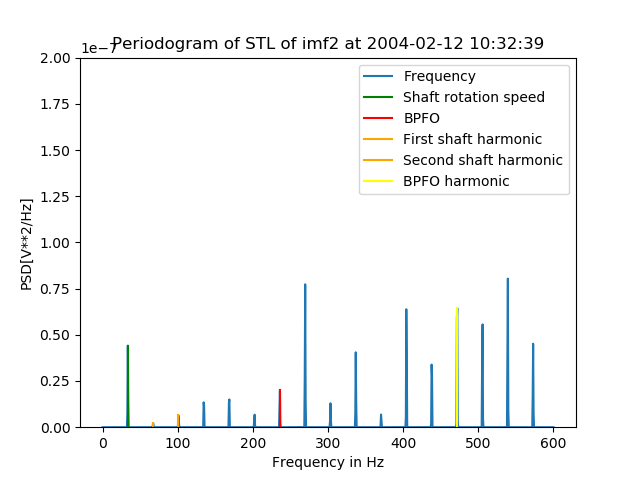
\includegraphics[width=0.8\linewidth]{../fig/periodogram_bpfo/start_imf2_bpfo}
	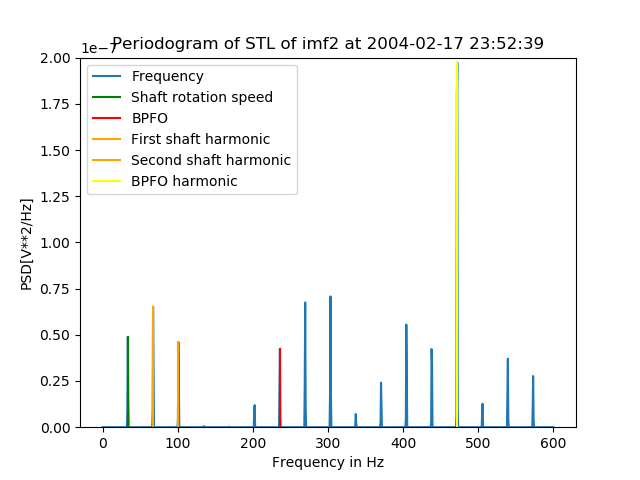
\includegraphics[width=0.8\linewidth]{../fig/periodogram_bpfo/end_imf2_bpfo}
	\caption{Periodogram of the pulse signal obtained from the second IMF, at the beginning (top) and the end (bottom) of experiment number 2.}
	\label{fig:startimf2bpfo}
\end{figure}

 \begin{figure}[H]
	\centering
	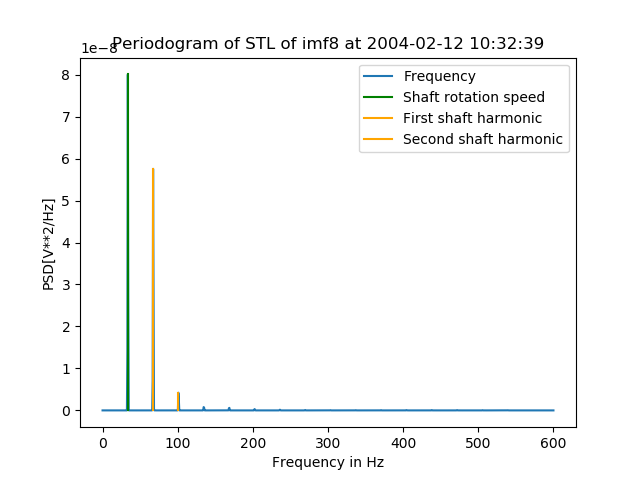
\includegraphics[width=0.8\linewidth]{../fig/periodogram_bpfo/start_imf8_shaft}
	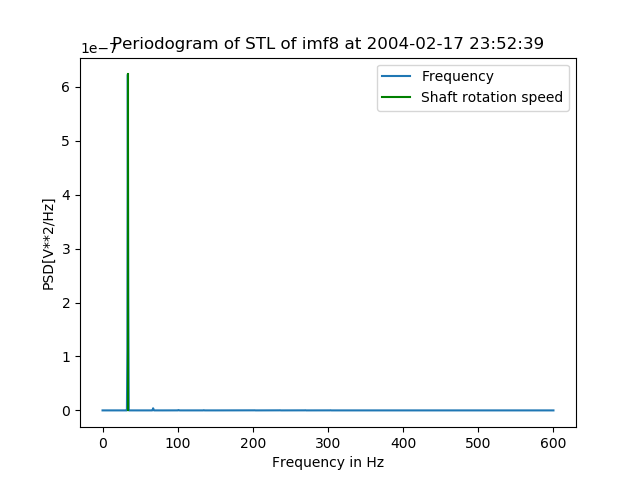
\includegraphics[width=0.8\linewidth]{../fig/periodogram_bpfo/end_imf8_shaft}
	\caption{Periodogram of the pulse signal obtained from IMF number 8, at the beginning (top) and the end (bottom) of experiment number 2.}
	\label{fig:startimf8shaft}
\end{figure}
\justify
\subsubsection{ Ball pass inner race frequency detection }

\begin{figure}[H]
	\centering
	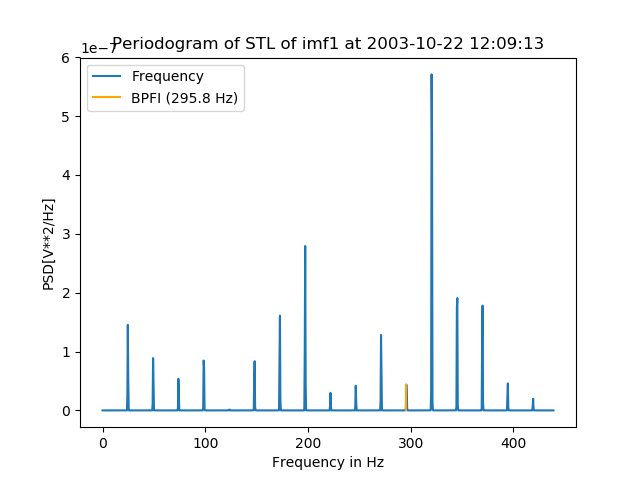
\includegraphics[width=0.8\linewidth]{../fig/periodogram_bpfi/start_imf1_bpfi}
	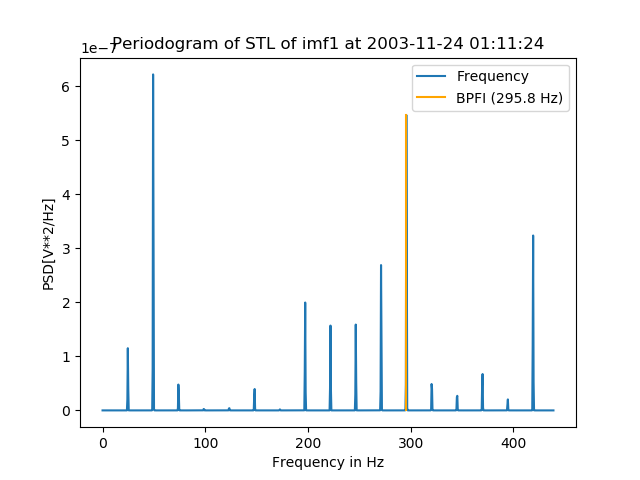
\includegraphics[width=0.8\linewidth]{../fig/periodogram_bpfi/end_imf1_bpfi}
	\caption{Periodogram of the pulse signal obtained from IMF number 1, at the beginning (top) and the end (bottom) of experiment number 1.}
	\label{fig:startimf1bpfi}
\end{figure}
\justify
Figure \ref{fig:startimf1bpfi} shows the periodograms obtained from the pulse signals of the first intrinsic mode functions at the start (top) and at the end (bottom) of experiment number 1. The inner race defect frequency is visible in both cases.
However, the shaft frequency is not visible. The difference between the theoretical value of the BPFI (296.8 Hz) and the detected value (295.8) is about 0.33 $\%$.
\section{Summary}
\label{sec:limitation}
The proposed method consists of transforming a vibration signal to a pulse like signal, which contains all diagnostics information in terms of bearing failure detection. In particular, the outer race and the inner race defect. The present method uses the empirical mode decomposition (EMD), followed by the seasonal trend decomposition method based on Loess (STL). The former is a signal decomposition method suited for non stationary and non linear signal, while the letter extracts periodic components from a signal.
\justify
Together they are able to generate a noise less periodogram which contains relevant frequency information for bearing fault detection. The periodogram approximates the power spectral density (PSD) of a signal. The PSD is the energy distribution of frequencies components of a signal.
By applying the proposed method, it was possible to identify conspicuous outer and inner race defect frequencies, as well as the roation frequency of the machine shaft, in a periodogram pertaining to a bearing undergoing failure.








\blankpage
\end{document}

